\documentclass[12pt]{article}
%\usepackage{amsmath}
\usepackage{graphicx}
%\usepackage{enumerate}
%\usepackage{natbib} %comment out if you do not have the package
\usepackage{url} % not crucial - just used below for the URL 

\usepackage[utf8]{inputenc}
\usepackage{amsfonts}
\usepackage{amsmath}
\usepackage{amssymb}
\usepackage[english]{babel}
\usepackage{bbm}
\usepackage{csquotes}
\usepackage{relsize}
\usepackage{todonotes}

\usepackage[
backend=biber,
style=alphabetic,
sorting=ynt
]{biblatex}

\addbibresource{sequential-sensitivity.bib}


%\pdfminorversion=4
% NOTE: To produce blinded version, replace "0" with "1" below.
\newcommand{\blind}{0}

% DON'T change margins - should be 1 inch all around.
\addtolength{\oddsidemargin}{-.5in}%
\addtolength{\evensidemargin}{-.5in}%
\addtolength{\textwidth}{1in}%
\addtolength{\textheight}{1.3in}%
\addtolength{\topmargin}{-.8in}%


\begin{document}

%\bibliographystyle{natbib}

\def\spacingset#1{\renewcommand{\baselinestretch}%
{#1}\small\normalsize} \spacingset{1}


%%%%%%%%%%%%%%%%%%%%%%%%%%%%%%%%%%%%%%%%%%%%%%%%%%%%%%%%%%%%%%%%%%%%%%%%%%%%%%

\if0\blind
{
  \title{\bf Adaptively Iterating Variance-Based Sensitivity Analysis}
  \author{
    Brian\ W.\ Bush \\
    National Renewable Energy Laboratory, \\ \\
    Joanne Wendelberger \\
    Los Alamos National Laboratory, \\ \\
    Rebecca Hanes \\
    National Renewable Energy Laboratory
  }
  \maketitle
} \fi

\if1\blind
{
  \bigskip
  \bigskip
  \bigskip
  \begin{center}
    {\LARGE\bf Adaptively Iterating Variance-Based Sensitivity Analysis}
\end{center}
  \medskip
} \fi

\bigskip
\begin{abstract}
Inspired by the well-established variance-based methods for global sensitivity analysis, we develop a local total sensitivity index that decomposes the global total sensitivity conditions by independent variables. We employ this local sensitivity index in a new method of experimental design that sequentially and adaptively samples the domain of a multivariate function according to local contributions to the global variance. The method is demonstrated on a nonlinear toy model that has a three-dimensional domain and a three-dimensional codomain, but also on a complex, high-dimensional simulation of the production of bioproducts from biomass. \todo{\small 100 or fewer words.}
\end{abstract}

\noindent%
{\it Keywords:} \todo{\small 3 to 6 keywords, that do not appear in the title}
\vfill

\newpage
%%%% FIXME: Remove comment before submitting.
%%%%\spacingset{2} % DON'T change the spacing!


\section{Introduction}


\section{Background}


\section{Method}

We consider multivariate functions $\mathbf{Y} \left( \mathbf{X} \right)$ with $m$ independent variables $X_i$ and $n$ dependent variables $Y_j$. (Table~\ref{tab:notation} summarizes the notation used in this paper.) These functions may represent the input-output relationship of computer models (either deterministic or stochastic) or physical experiments.

We approach the problem of developing local versions of variable-based global sensitivity indices by expressing the standard global indices \cite{saltelli_variance_2010} in forms amenable to local decomposition. The local total sensitivity separately partitions the global sensitivity along each independent variable. We then adopt experimental designs that are suitable for iterative extension. The iterative experimental design samples the space of independent variables proportionally to the local variance indices observed so far in the experiment.

\begin{table}
    \centering
    \begin{tabular}{ll}
        Symbol & Definition \\
        \hline
        $i \in \{1 \ldots m\}$ & independent-variable index and dimension \\
        $j \in \{1 \ldots n\}$ & dependent-variable index and dimension \\
        $k \in \{1 \ldots N\}$ & observation index and dimension \\
        $\mathbb{E}_Z$ & expectation over random variable(s) $Z \in \{ X_i, \mathbf{X}_{\sim i} \}$ \\
        $\mathbb{V}_Z$ & variance over random variable(s) $Z \in \{ X_i, \mathbf{X}_{\sim i} \}$ \\
        $X_i \in [0, 1]$ & independent variable for dimension $i$ \\
        $\mathbf{X}_{\sim i}$ & independent variables except for dimension $i$ \\
        $Y_j$ & dependent variable for dimension $j$ \\
        $\mathbf{A}$, $\mathbf{B}$ & $N \times k$ design matrices \\
        $\mathbf{A}_{\mathbf{B}_i}$ & design matrix $\mathbf{A}$ with its $i$th column replaced \\ & by the $i$th column of $\mathbf{B}$ \\
        $x_{\mathbf{Z}_i}^{(k)} \in [0, 1]$ & $i$th independent variable for the $k$th observation \\ & in the design matrix $\mathbf{Z} \in \{ \mathbf{A}, \mathbf{B} \}$ \\
        $y_{\mathbf{Z},j}^{(k)}$ & $j$th dependent variable for the $k$th observation \\ & using the design matrix $\mathbf{Z} \in \{ \mathbf{A}, \mathbf{B}, \mathbf{A}_{\mathbf{B}_i} \}$ \\
        $\mathbbm{1}_c$ & indicator function: $1$ if the condition $c$ holds, \\ & but $0$ otherwise \\
        $u \mathrel{\hat=} v$ & $v$ is an estimate for $u$ \\
    \end{tabular}
    \caption{Notation used in this paper, inspired by and generally consistent with \cite{saltelli_variance_2010}.}
    \label{tab:notation}
\end{table}


\subsection{Global Sensitivity}

We start from standard definitions \cite{saltelli_variance_2010} that use conditional expectations and variances to express the first-order and total sensitivity indices, respectively:
\begin{align}
    S_{i,j} & = \frac{\mathbb{V}_{X_i} \left[ \mathbb{E}_{\mathbf{X}_{\sim i}} \left[ Y_j \middle| X_i \right] \right]}{\mathbb{V}_\mathbf{X} \left[ Y_j \right]} \label{eq:satellis}
    \\
    T_{i,j} & = \frac{\mathbb{E}_{\mathbf{X}_{\sim i}} \left[ \mathbb{V}_{X_i} \left[ Y_j \middle| \mathbf{X}_{\sim i} \right] \right]}{\mathbb{V}_\mathbf{X} \left[ Y_j \right]} \label{eq:saltellit}
\end{align}
The first-order index $S_{i,j}$ quantifies the influence of $X_i$ solely upon the variance of $Y_j$ whereas the total index $T_{i,j}$ quantifies the influence of $X_i$ in combination with other independent variables upon the variance of $Y_j$. The two indices arise from decomposing the variance $Y_j$ and obey a variety of summation relationships and bounds---see [cite]\todo{Cite Saltelli books and review papers.} for detailed discussion.

Practically estimating Eqs.~(\ref{eq:satellis}) and~(\ref{eq:saltellit}) may be problematic because of computational complexity, finite sample size, and numerical issues. Careful design of experiments alleviates some of these difficulties. An efficient design employs two $N \times k$ design matrices, $\mathbf{A}$ and $\mathbf{B}$, that are hybridized into matrices $\mathbf{A}_{\mathbf{B}_i}$ that are constructed by replacing the $i$th column of $\mathbf{A}$ with the $i$th column of $\mathbf{B}$. The number of rows $N$ determines the size of the experiment, which requires evaluating $\mathbf{Y}\left(\mathbf{X}\right)$ for each row of $\mathbf{A}$, $\mathbf{B}$, and $\mathbf{A}_{\mathbf{B}_i}$: thus $N (k + 2)$ observations must be made. The column-swapping construction facilitates efficient evaluation of the conditional expectations and variances by controlling which independent variables are varied and by organizing the computation.

The best-practice recommendations of Saltelli~\cite{saltelli_variance_2010} are to use the formulae in Jansen~\cite{jansen_analysis_1999} when computing the variances of conditional expectations and the expectations of conditional variances:
\begin{align}
    \mathbb{V}_\mathbf{X} \left[ Y_j \right] - \mathbb{V}_{X_i} \left[ \mathbb{E}_{\mathbf{X}_{\sim i}} \left[ Y_j \middle| X_i \right] \right] & \mathrel{\hat=} \frac{1}{2 N} \sum_{k=1}^N \left| y_{\mathbf{B},j}^{(k)} - y_{\mathbf{A}_{\mathbf{B}_i},j}^{(k)} \right|^2 \label{eq:jansens}
    \\
    \mathbb{E}_{\mathbf{X}_{\sim i}} \left[ \mathbb{V}_{X_i} \left[ Y_j \middle| \mathbf{X}_{\sim i} \right] \right] & \mathrel{\hat=} \frac{1}{2 N} \sum_{k=1}^N \left| y_{\mathbf{A},j}^{(k)} - y_{\mathbf{A}_{\mathbf{B}_i},j}^{(k)} \right|^2 \label{eq:jansent}
\end{align}
Here the $y_{\mathbf{A},j}^{(k)}$, $y_{\mathbf{B},j}^{(k)}$, and $y_{\mathbf{A}_{\mathbf{B}_i},j}^{(k)}$ are the observation of $Y_j$ for the $k$th row of the design matrix $\mathbf{A}$, $\mathbf{B}$, and $\mathbf{A}_{\mathbf{B}_i}$, respectively. We supplement these formulae with the analogous formula for computing the overall variance:
\begin{equation}
    \mathbb{V}_\mathbf{X} \left[ Y_j \right] \mathrel{\hat=} \frac{1}{2 N} \sum_{k=1}^N \left| y_{\mathbf{A},j}^{(k)} - y_{\mathbf{B},j}^{(k)} \right|^2 \label{eq:jansenv}
\end{equation}

Combining Eqs.~(\ref{eq:jansens}) through (\ref{eq:jansenv}), we adopt the following estimators for first-order and total global sensitivities and variance:
\begin{align}
    \hat{S}_{i,j} = 1 - & \frac{\sum_{k=1}^N \left| y_{\mathbf{B},j}^{(k)} - y_{\mathbf{A}_{\mathbf{B}_i},j}^{(k)} \right|^2}{\sum_{k=1}^N \left| y_{\mathbf{A},j}^{(k)} - y_{\mathbf{B},j}^{(k)} \right|^2} \label{eq:ours}
    \\
    \hat{T}_{i,j} = & \frac{\sum_{k=1}^N \left| y_{\mathbf{A},j}^{(k)} - y_{\mathbf{A}_{\mathbf{B}_i},j}^{(k)} \right|^2}{\sum_{k=1}^N \left| y_{\mathbf{A},j}^{(k)} - y_{\mathbf{B},j}^{(k)} \right|^2} \label{eq:ourt}
    \\
    \hat{V}_{j} = & \frac{1}{2 N} \sum_{k=1}^N \left| y_{\mathbf{A},j}^{(k)} - y_{\mathbf{B},j}^{(k)} \right|^2 \label{eq:ourv}
\end{align}


\subsection{Experimental Design}

Although any of a number of design methods could be used for creating the $\mathbf{A}$ and $\mathbf{B}$ matrices, quasi-random sequences are well suited for computing the sensitivity indices and Ref.~\cite{saltelli_variance_2010} recommends using Sobol' sequences because of their low discrepancy properties. In this procedure, the $\mathbf{A}$ and $\mathbf{B}$ matrices are placed side-by-side to form an $N \times 2 k$ matrix where the $N$ rows are consecutive points in the $2 k$-dimensional Sobol' sequence. An experiment can very simply be enlarged just by appending additional rows of the Sobol' sequence, so this design procedure is well suited for iteratively extending a sensitivity analysis.

Without loss of generality, we require that the domain of each independent variable be $[0, 1]$. This is convenient because the range of the Sobol' sequence is also $[0, 1]$ in each dimension.


\subsection{Local Sensitivity}

In developing a local version of variance-based sensitivity, one would like to attribute the variance in output to a specific value or interval of the independent variables. Equation~(\ref{eq:ourt}), for example, involves evaluating $Y_j$ at the points $x_{\mathbf{A}_i}^{(k)}$ and $x_{\mathbf{B}_i}^{(k)}$ to compute the contribution $\left| y_{\mathbf{A},j}^{(k)} - y_{\mathbf{A}_{\mathbf{B}_i},j}^{(k)} \right| ^2$ to the global total sensitivity. For lack of a more specific way to assign this contribution to a particular value of the independent variable, we can simply spread this contribution uniformly between $x_{\mathbf{A}_i}^{(k)}$ and $x_{\mathbf{B}_i}^{(k)}$. Thus we define $t_{i,j}^{(\alpha,\epsilon)}(x_i)$ to be the local sensitivity of the output $y_j$ upon the input $x_i$:
\begin{equation}
    t_{i,j}^{(\alpha,\epsilon)}(x) = \mathlarger{\mathlarger{\sum}}_{k=1}^N \left| y_{\mathbf{A},j}^{(k)} - y_{\mathbf{A}_{\mathbf{B}_i},j}^{(k)} \right| ^ \alpha  \cdot \frac{\mathbbm{1}_{\min \left\{ x_{\mathbf{A}_i}^{(k)} , x_{\mathbf{B}_i}^{(k)} \right\} - \frac{\epsilon}{2} \leq x \leq \max \left\{ x_{\mathbf{A}_i}^{(k)} , x_{\mathbf{B}_i}^{(k)} \right\} + \frac{\epsilon}{2}}}{\left| x_{\mathbf{A}_i}^{(k)} - x_{\mathbf{B}_i}^{(k)} + \epsilon \right|} \label{eq:tx}
\end{equation}
Here we have introduced $\epsilon > 0$ to guard against division by zero, which could occur if the two $x_i$ coincide, and we have replaced the exponent $2$ by the general parameter $\alpha$. The parameter $\alpha$ amplifies the difference between the dependent variables, with $\alpha = 2$ corresponding to computing the variance. The parameter $\epsilon$ slightly widens the interval over which the contribution to the variance is spread. It is also useful to define a cumulative version of the local sensitivity:
\begin{equation}
    T_{i,j}^{(\alpha,\epsilon)}(x) = \frac{1}{2 N \hat{V}_j} \int_{-\infty}^x d x^\prime \; t_{i,j}^{(\alpha,\epsilon)}(x^\prime) \label{eq:cumt}
\end{equation}
Note that we can recover the global total sensitivity index, Equation (\ref{eq:ourt}), from the limit of Equation (\ref{eq:cumt}):
\begin{equation*}
    \hat{T}_{i,j} = \lim_{x \rightarrow \infty} T_{i,j}^{(2,\epsilon)}(x)
\end{equation*}

In order to sample an independent variable proportionally to $t_{i,j}^{(\alpha,\epsilon)}(x_i)$, we need a normalized version of it, which we call the sensitivity density:
\begin{equation}
    \tau_{i,j}^{(\alpha,\epsilon)}(x) = \left. \frac{t_{i,j}^{(\alpha,\epsilon)}(x)}{t_{i,j}^{(0,\epsilon)}(x)} \middle/ \int_{-\infty}^{\infty} d x^\prime \; \frac{t_{i,j}^{(\alpha,\epsilon)}(x^\prime)}{t_{i,j}^{(0,\epsilon)}(x^\prime)} \right. \label{eq:taux}
\end{equation}
The factor $t_{i,j}^{(0,\epsilon)}(x)$ in the denominators removes the non-uniformity in the sampling of $x_i$. Finally, we can further summarize the local sensitivity by averaging it over the $n$ dependent variables; we call this the average sensitivity density:
\begin{equation}
    \overline{\tau}_i^{(\alpha,\epsilon)}(x) = \frac{1}{n} \sum_{j=1}^n \tau_{i,j}^{(\alpha,\epsilon)}(x) \label{eq:taubar}
\end{equation}
It also has a cumulative version:
\begin{equation}
    \overline{T}_i^{(\alpha,\epsilon)}(x) = \int_{-\infty}^x d x^\prime \; \overline{\tau}_i^{(\alpha,\epsilon)}(x^\prime) \label{eq:tbar}
\end{equation}

Unfortunately, the expression of the first-order sensitivity in Eq.~(\ref{eq:ours}) as the difference of two terms precludes its analogous decomposition into a local first-order sensitivity index. One could create a local first-order \textit{insensitivity} index based on $1 - \hat{S}_{i,j}$, but the density of insensitivity would not be practical for iteratively adapting experimental designs.

\subsection{Adaptively Iterating Sensitivity Analysis}

We are now in a position to specify an algorithm for iteratively adapting the experimental design for a sensitivity analysis as that analysis proceeds. Let $M$ be the batch size for the iterations.
\begin{enumerate}
    \item Evaluate $y_{\mathbf{A},j}^{(k)}$, $y_{\mathbf{B},j}^{(k)}$, and $y_{\mathbf{A}_{\mathbf{B}_i},j}^{(k)}$ for the first $M$ rows of the design matrices $\mathbf{A}$, $\mathbf{B}$, and $\mathbf{A}_{\mathbf{B}_i}$.
    \item Compute the cumulative average sensitivity densities $\overline{T}_i^{(\alpha,\epsilon)}(x)$ for each independent variable.
    \item Append $M$ rows to the design matrices by taking the next $M$ points in the Sobol' sequence, but transform those points according to the average sensitivity density. Namely, the Sobol' point $s_\ell$ is mapped to ${\overline{T}_i^{(\alpha,\epsilon)}}^{-1}(s_\ell)$, where $i = 1 + (\ell - 1 \mod m)$, since $\ell \in \{ 1 \ldots 2 m \}$ because the $\mathbf{A}$ and $\mathbf{B}$ matrices are placed side-by-side in the Sobol' space.
    \item Evaluate $y_{\mathbf{A},j}^{(k)}$, $y_{\mathbf{B},j}^{(k)}$, and $y_{\mathbf{A}_{\mathbf{B}_i},j}^{(k)}$ for these $M$ new rows of the design matrix.
    \item Proceed to step \#2 above.
\end{enumerate}
For computational efficiency, the $\hat{V}_j$ and $T_{i,j}^{(\alpha,\epsilon)}(x)$ can be updated during each iteration instead of being computed from scratch. The batch size can be $M = 1$ if an online algorithm is desired. The parameter $\epsilon$ should be set to a small positive value. The parameter $\alpha$ allows one to make the sampling completely non-adapative ($\alpha = 0$) or highly adaptive (large positive $\alpha$): setting $\alpha$ too high may result in missing sensitivities in the input space if the batch size is too small, since the algorithm may home in on the first observed region of sensitivity, thus missing other areas of high sensitivity.


\subsection{Functional PCA}

\todo{Hybridize the method with functional PCA.}


\section{Results}

We evaluate the adaptive iterative approach to sensitivity analysis first using a toy model with a manageably small number of dimensions, and then with a complex simulation.


\subsection{Toy Model}

The Appendix~\ref{sec:toy} describes a class of toy models that have strong nonlinearities, configurable dimensionality, and specifiable discontinuities in the dependent variables. For convenience in exploring and plotting results, we select three input dimensions ($m = 3$) and three output dimensions ($n = 3$). The model has a zeroth-order discontinuity in the output at $x_1 \doteq 0.59$, a first-order discontinuity in the output at $x_2 \doteq 0.95$, and a second-order discontinuity in the output at $x_3 \doteq 0.10$.

Table~\ref{tab:toyglobal} shows that the global sensitivities when $N = M = 1000$ exhibit a diversity of sensitive and insensitive first-order and total sensitivity indices. The cumulative sensitivities $T_{i,j}^{(2,\epsilon)}(x)$ in Figure~\ref{fig:toy-tx} approach the global sensitivities $\hat{T}_{i,j}$ of Table~\ref{tab:toyglobal} as $x_i \rightarrow 1$. One can also see mild nonlinearities near the $x_1 \doteq 0.59$, and $x_3 \doteq 0.10$ discontinuities of the model. The local sensitivity density in Figure~\ref{fig:toy-tau} highlights the stronger contributions to the local variance near the model's zeroth- and first-order discontinuities ($x_1 \doteq 0.59$ and $x_2 \doteq 0.95$). Averaging over the output dimensions yields the average local sensitivity density in Figure~\ref{fig:toy-taubar}. Figure~\ref{fig:toy-density} shows how densely different regions are sampled in the first five batches of $M = 10$ observations when the sensitivity analysis proceeds adaptively:\ this illustrates how quickly the algorithm detects the areas of higher variance as it transitions from the initial uniform sampling to the sensitivity-emphasizing sampling. Furthermore, Figure~\ref{fig:toy-sample} displays two-dimensional projections of actual sampling for a batch size of $M = 10$, with 100 batches so $N = 1000$: one can see that the algorithm explores the whole space while concentrating on areas of high sensitivity.

\begin{figure}
    \centering
    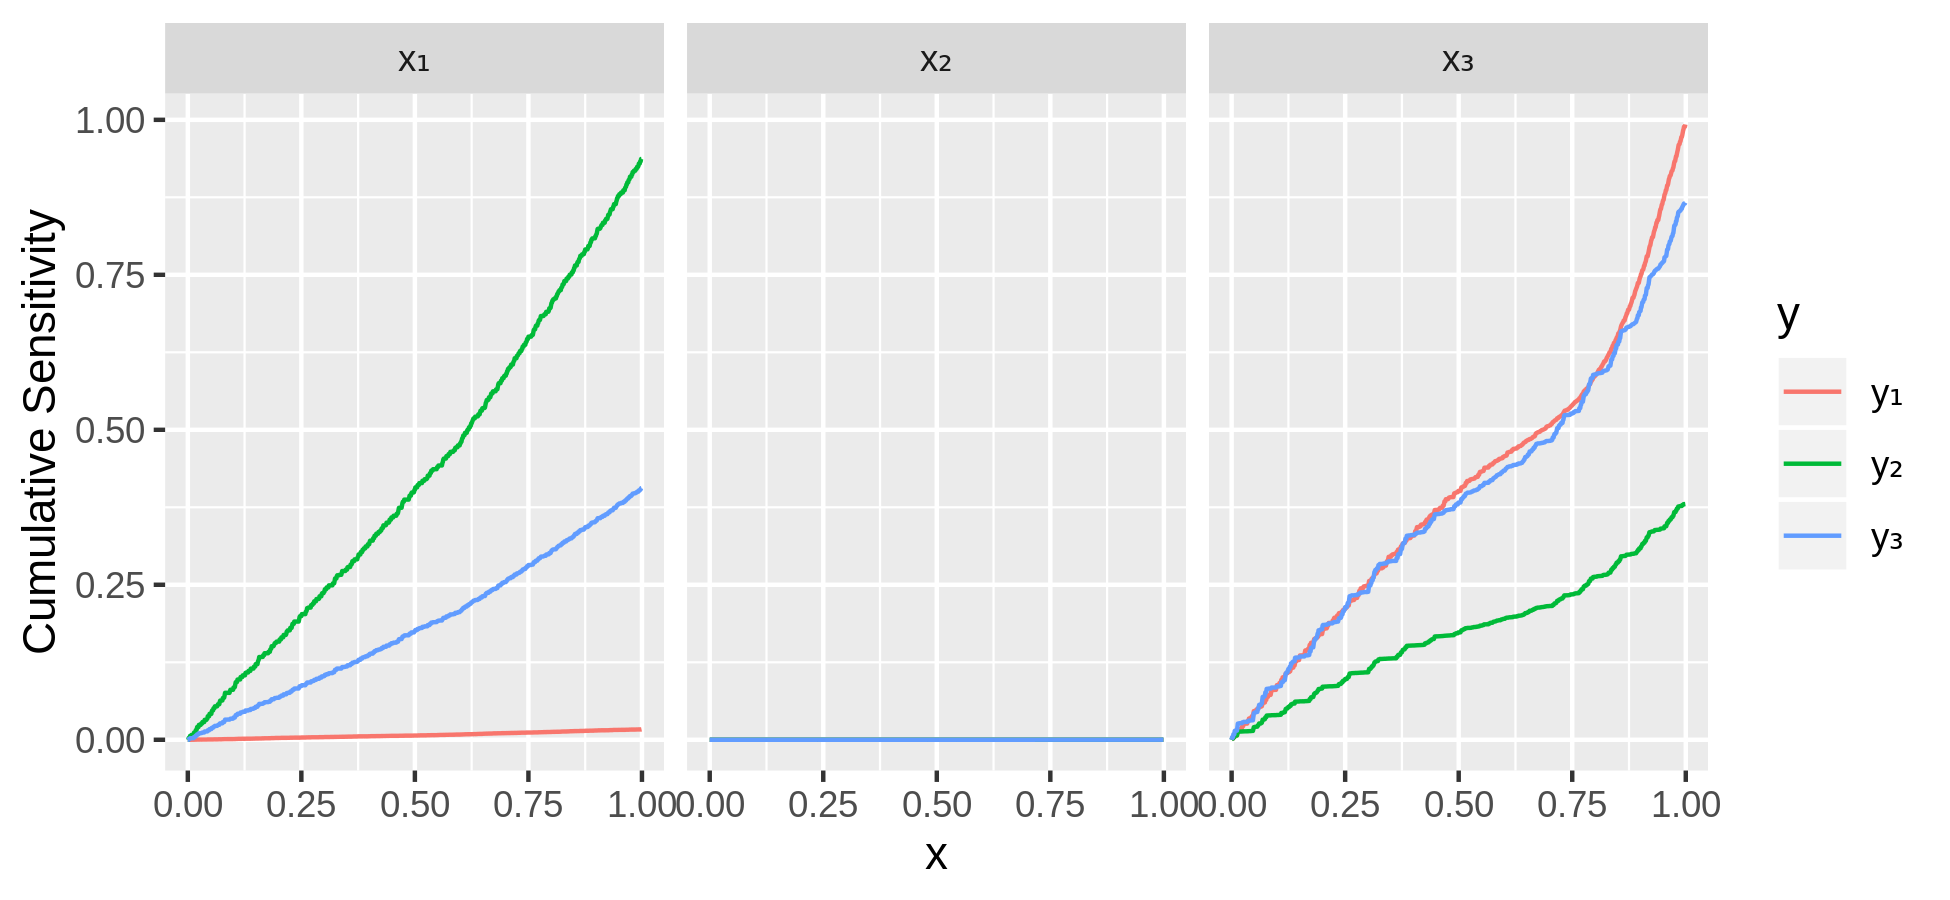
\includegraphics[width=1.00\linewidth]{figures/toy-tx.png}
    \caption{Cumulative local sensitivity $T_{i,j}^{(2,\epsilon)}(x)$ for the toy model, with $\epsilon = 10^{-4}$ and $N = M = 1000$.}
    \label{fig:toy-tx}
\end{figure}

\begin{table}
\centering
\begin{tabular}{l|c|c|c}
$\hat{S}_{i,j}$ & $x_1$ & $x_2$ & $x_3$ \\
\hline
$y_1$ & 0.01 & 0.00 & 0.98 \\
$y_2$ & 0.62 & 0.00 & 0.06 \\
$y_3$ & 0.13 & 0.00 & 0.59 \\
\end{tabular}
\quad
\begin{tabular}{l|c|c|c}
$\hat{T}_{i,j}$ & $x_1$ & $x_2$ & $x_3$ \\
\hline
$y_1$ & 0.01 & 0.00 & 0.99 \\
$y_2$ & 0.94 & 0.00 & 0.38 \\
$y_3$ & 0.41 & 0.00 & 0.87 \\
\end{tabular}
\caption{Global first-order sensitivity (left) and total sensitivities (right) results for the toy model, on a scale from zero (insensitive) to one (sensitive), with one large batch of observations $N = M = 1000$.}
\label{tab:toyglobal}
\end{table}

\begin{figure}
    \centering
    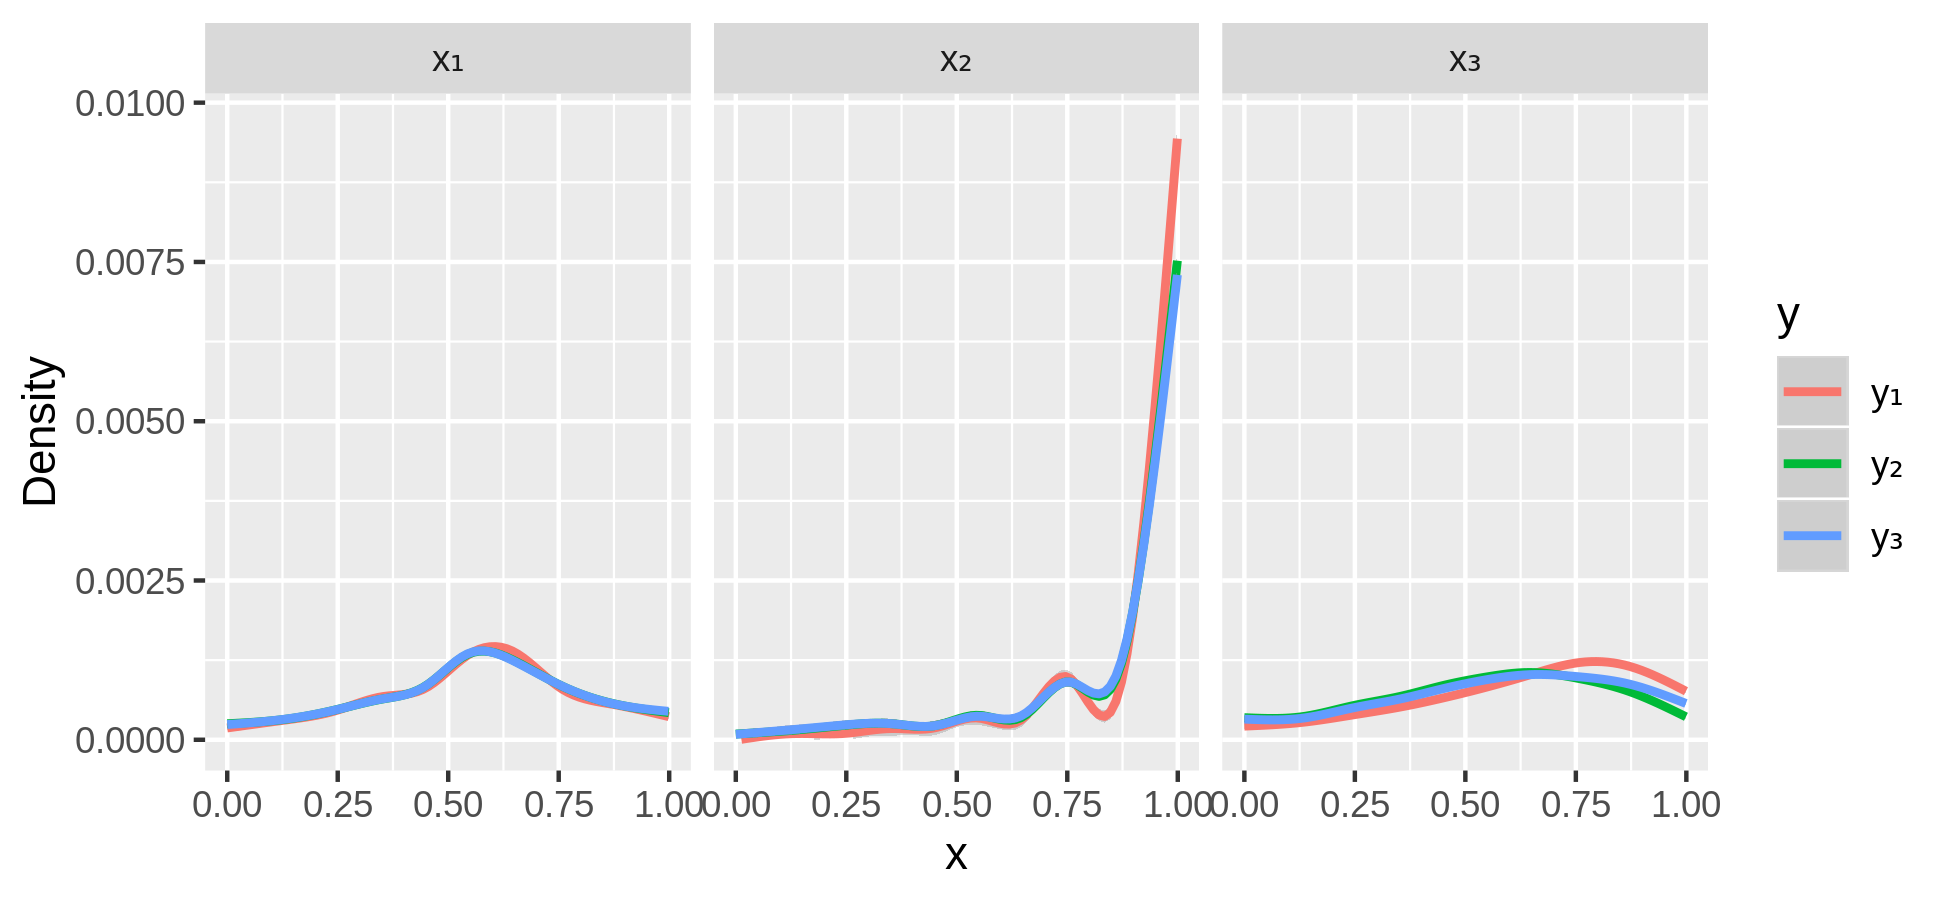
\includegraphics[width=1.00\linewidth]{figures/toy-tau.png}
    \caption{Sensitivity density $\tau_{i,j}^{(2,\epsilon)}(x)$ for the toy model, with $\epsilon = 10^{-4}$ and $N = M = 1000$. (Note that the density is smoothed using a general additive model.)}
    \label{fig:toy-tau}
\end{figure}

\begin{figure}
    \centering
    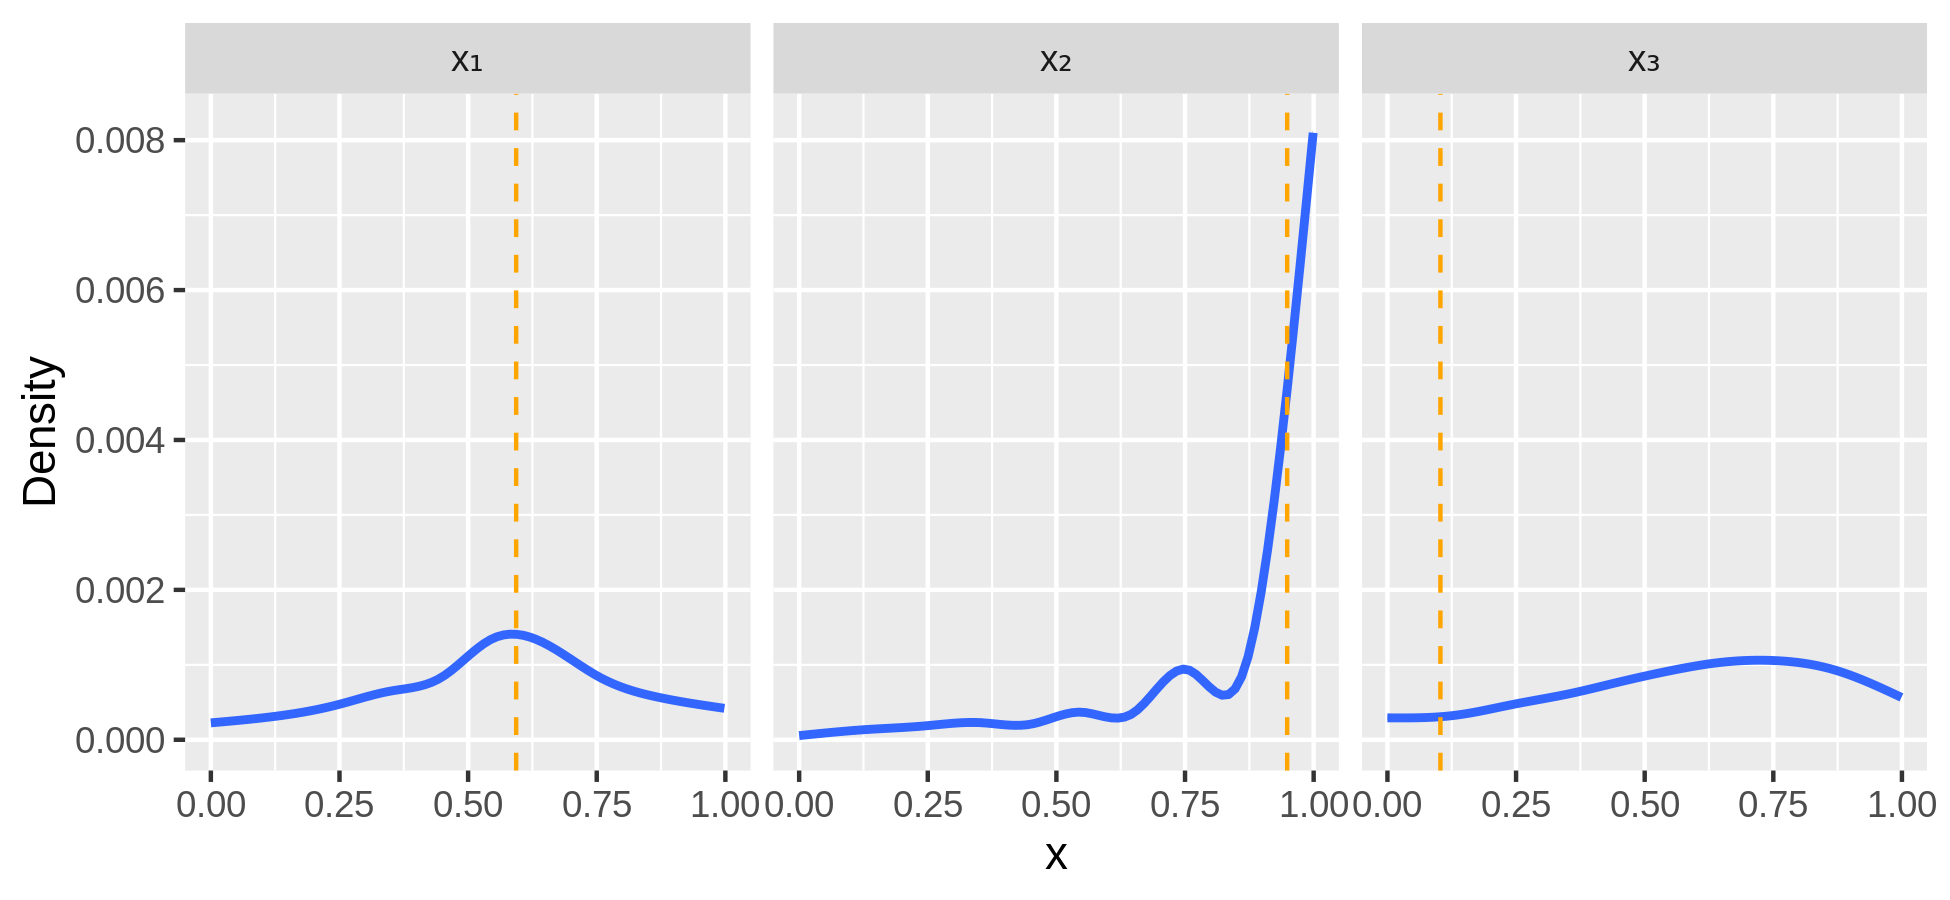
\includegraphics[width=1.00\linewidth]{figures/toy-taubar.png}
    \caption{Averaged sensitivity density $\overline{\tau}_i^{(2,\epsilon)}(x)$ for the toy model, with $\epsilon = 10^{-4}$ and $N = M = 1000$. The three dashed orange lines mark locations of the toy model's discontinuities with respect to its three independent variables: the algorithm successfully detects the zeroth- and first-order discontinuities in $x_1$ and $x_2$, respectively, but not the second-order discontinuity in $x_3$. (Note that the density is smoothed using a general additive model.)}
    \label{fig:toy-taubar}
\end{figure}

\begin{figure}
    \centering
    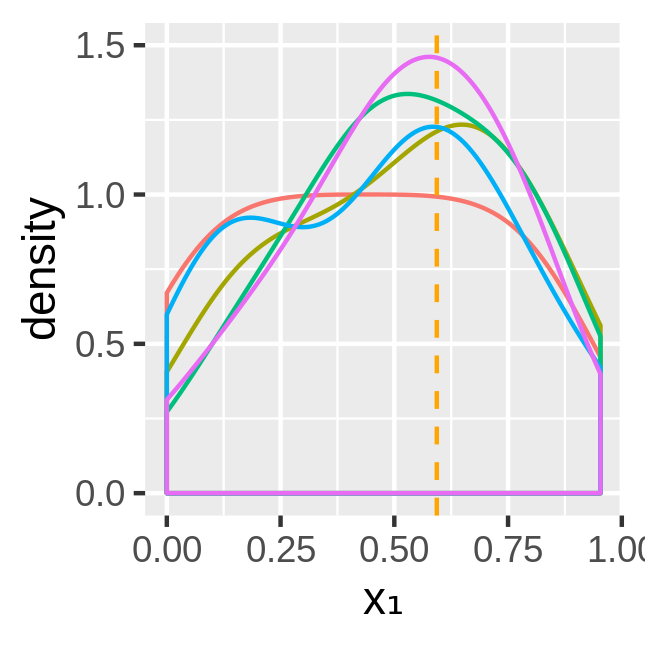
\includegraphics[width=0.300\linewidth]{figures/toy-density1.png}
    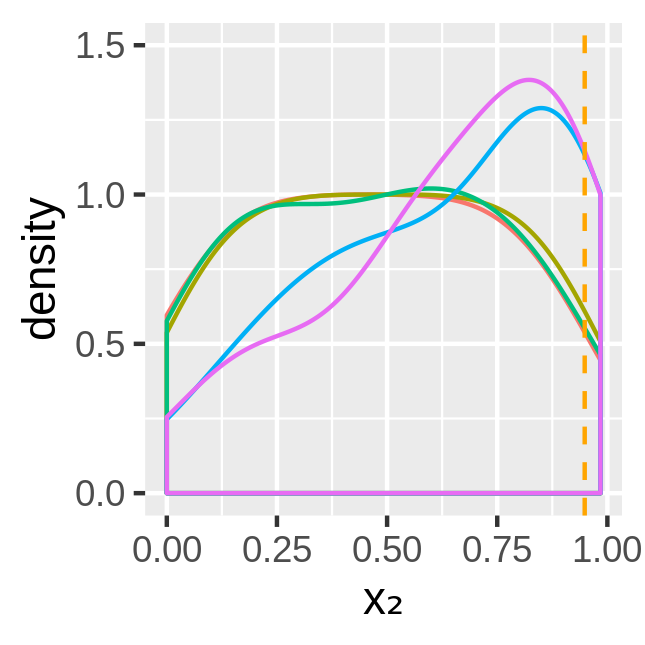
\includegraphics[width=0.300\linewidth]{figures/toy-density2.png}
    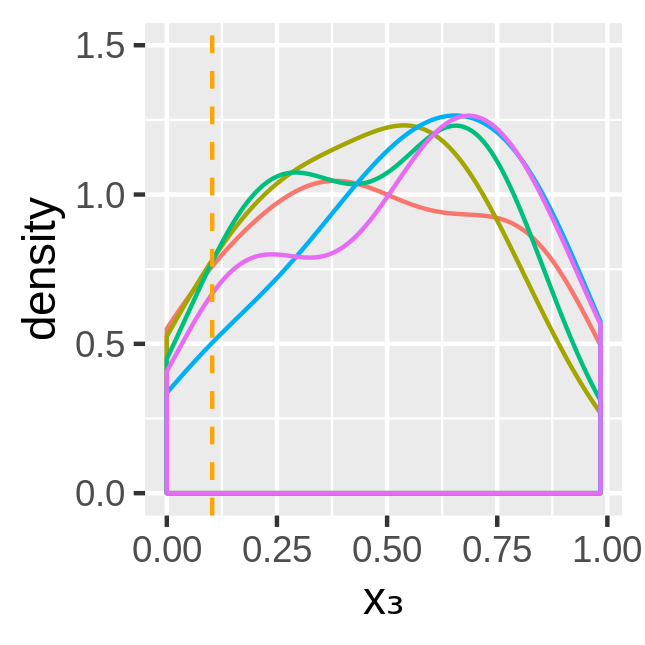
\includegraphics[width=0.300\linewidth]{figures/toy-density3.png}
    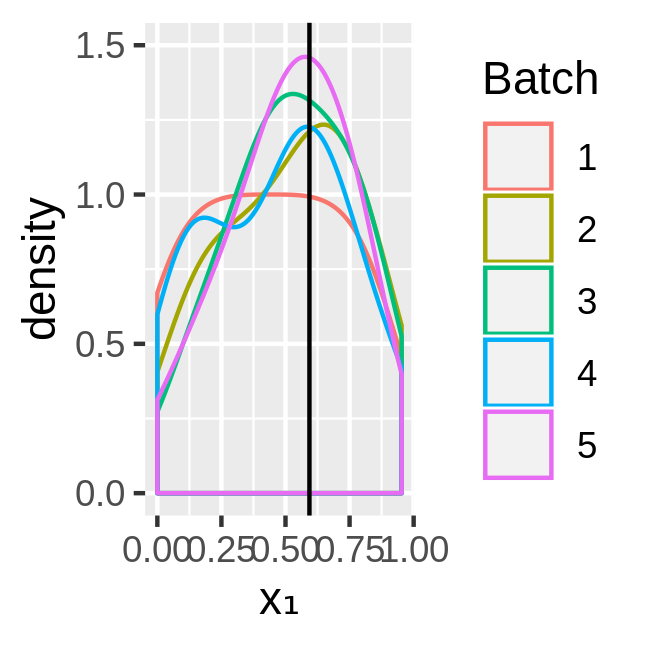
\includegraphics[width=0.075\linewidth,clip=true,trim={1.5in 0 2.15 2.15}]{figures/toy-density.png}
    \caption{Density of sampling in the first five batches of $M = 10$ observations in adaptive sampling according to $\overline{\tau}_i^{(2,\epsilon)}(x)$ for the toy model, with $\epsilon = 10^{-4}$, starting with a first batch that uniformly samples. The three dashed orange lines mark locations of the toy model's discontinuities with respect to its three independent variables: the algorithm successfully detects the zeroth- and first-order discontinuities in $x_1$ and $x_2$, respectively, but not the second-order discontinuity in $x_3$. (Note that the density is smoothed using a general additive model.)}
    \label{fig:toy-density}
\end{figure}

\begin{figure}
    \centering
    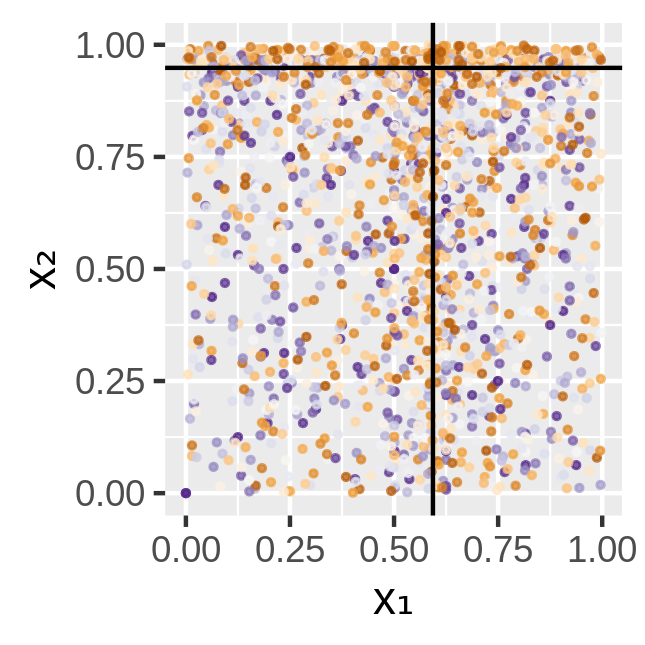
\includegraphics[width=0.300\linewidth]{figures/toy-sample12.png}
    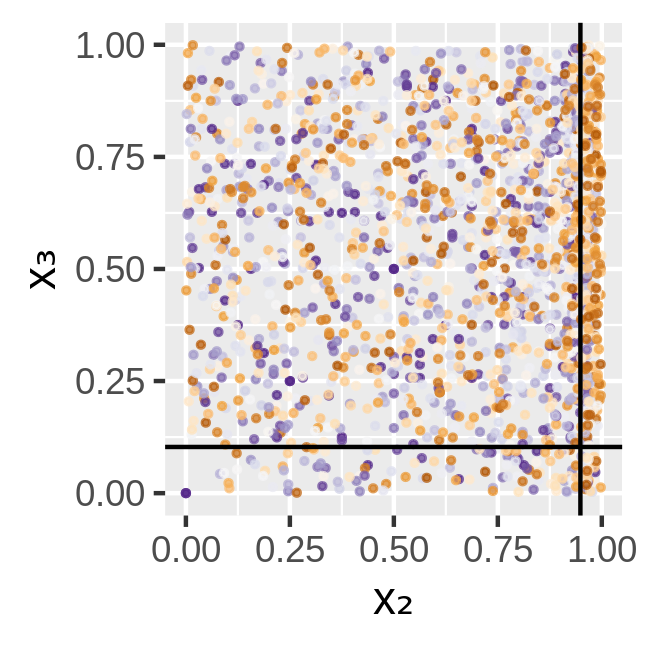
\includegraphics[width=0.300\linewidth]{figures/toy-sample23.png}
    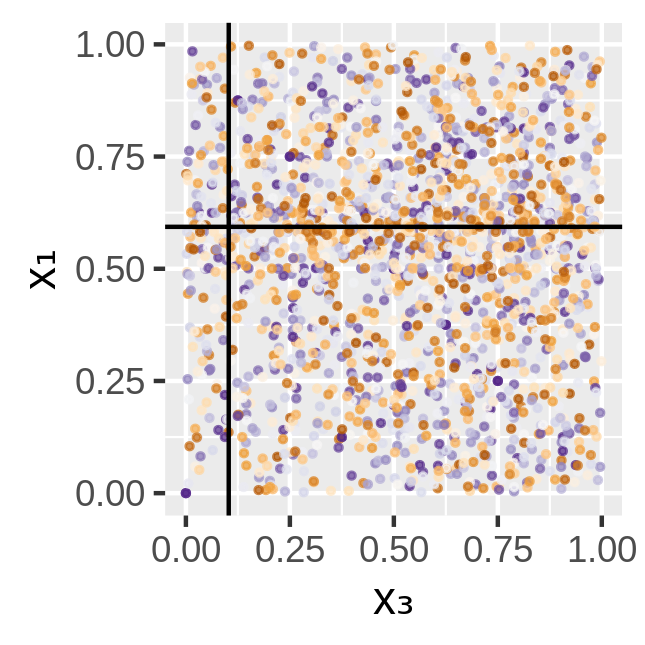
\includegraphics[width=0.300\linewidth]{figures/toy-sample31.png}
    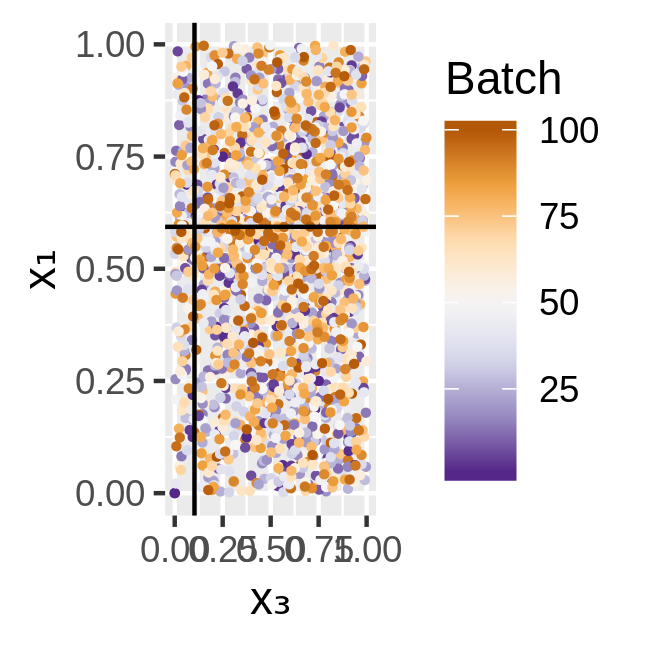
\includegraphics[width=0.075\linewidth,clip=true,trim={1.5in 0 2.15 2.15}]{figures/toy-sample.png}
    \caption{Two-dimensional projections of adaptive sampling according to $\overline{\tau}_i^{(2,\epsilon)}(x)$ for the toy model, with $\epsilon = 10^{-4}$ and for 100 sequential batches of $M = 10$ observations, so $N = 1000$. The solid black lines mark locations of the toy model's discontinuities with respect to its three independent variables: the algorithm successfully detects the zeroth- and first-order discontinuities in $x_1$ and $x_2$, respectively, but not the second-order discontinuity in $x_3$.}
    \label{fig:toy-sample}
\end{figure}


\subsection{Bioproduct Transition Dynamics Model}

Figure~\ref{fig:btd-t}
Figure~\ref{fig:btd-tau}
Figure~\ref{fig:btd-taubar1}

\begin{figure}
    \centering
    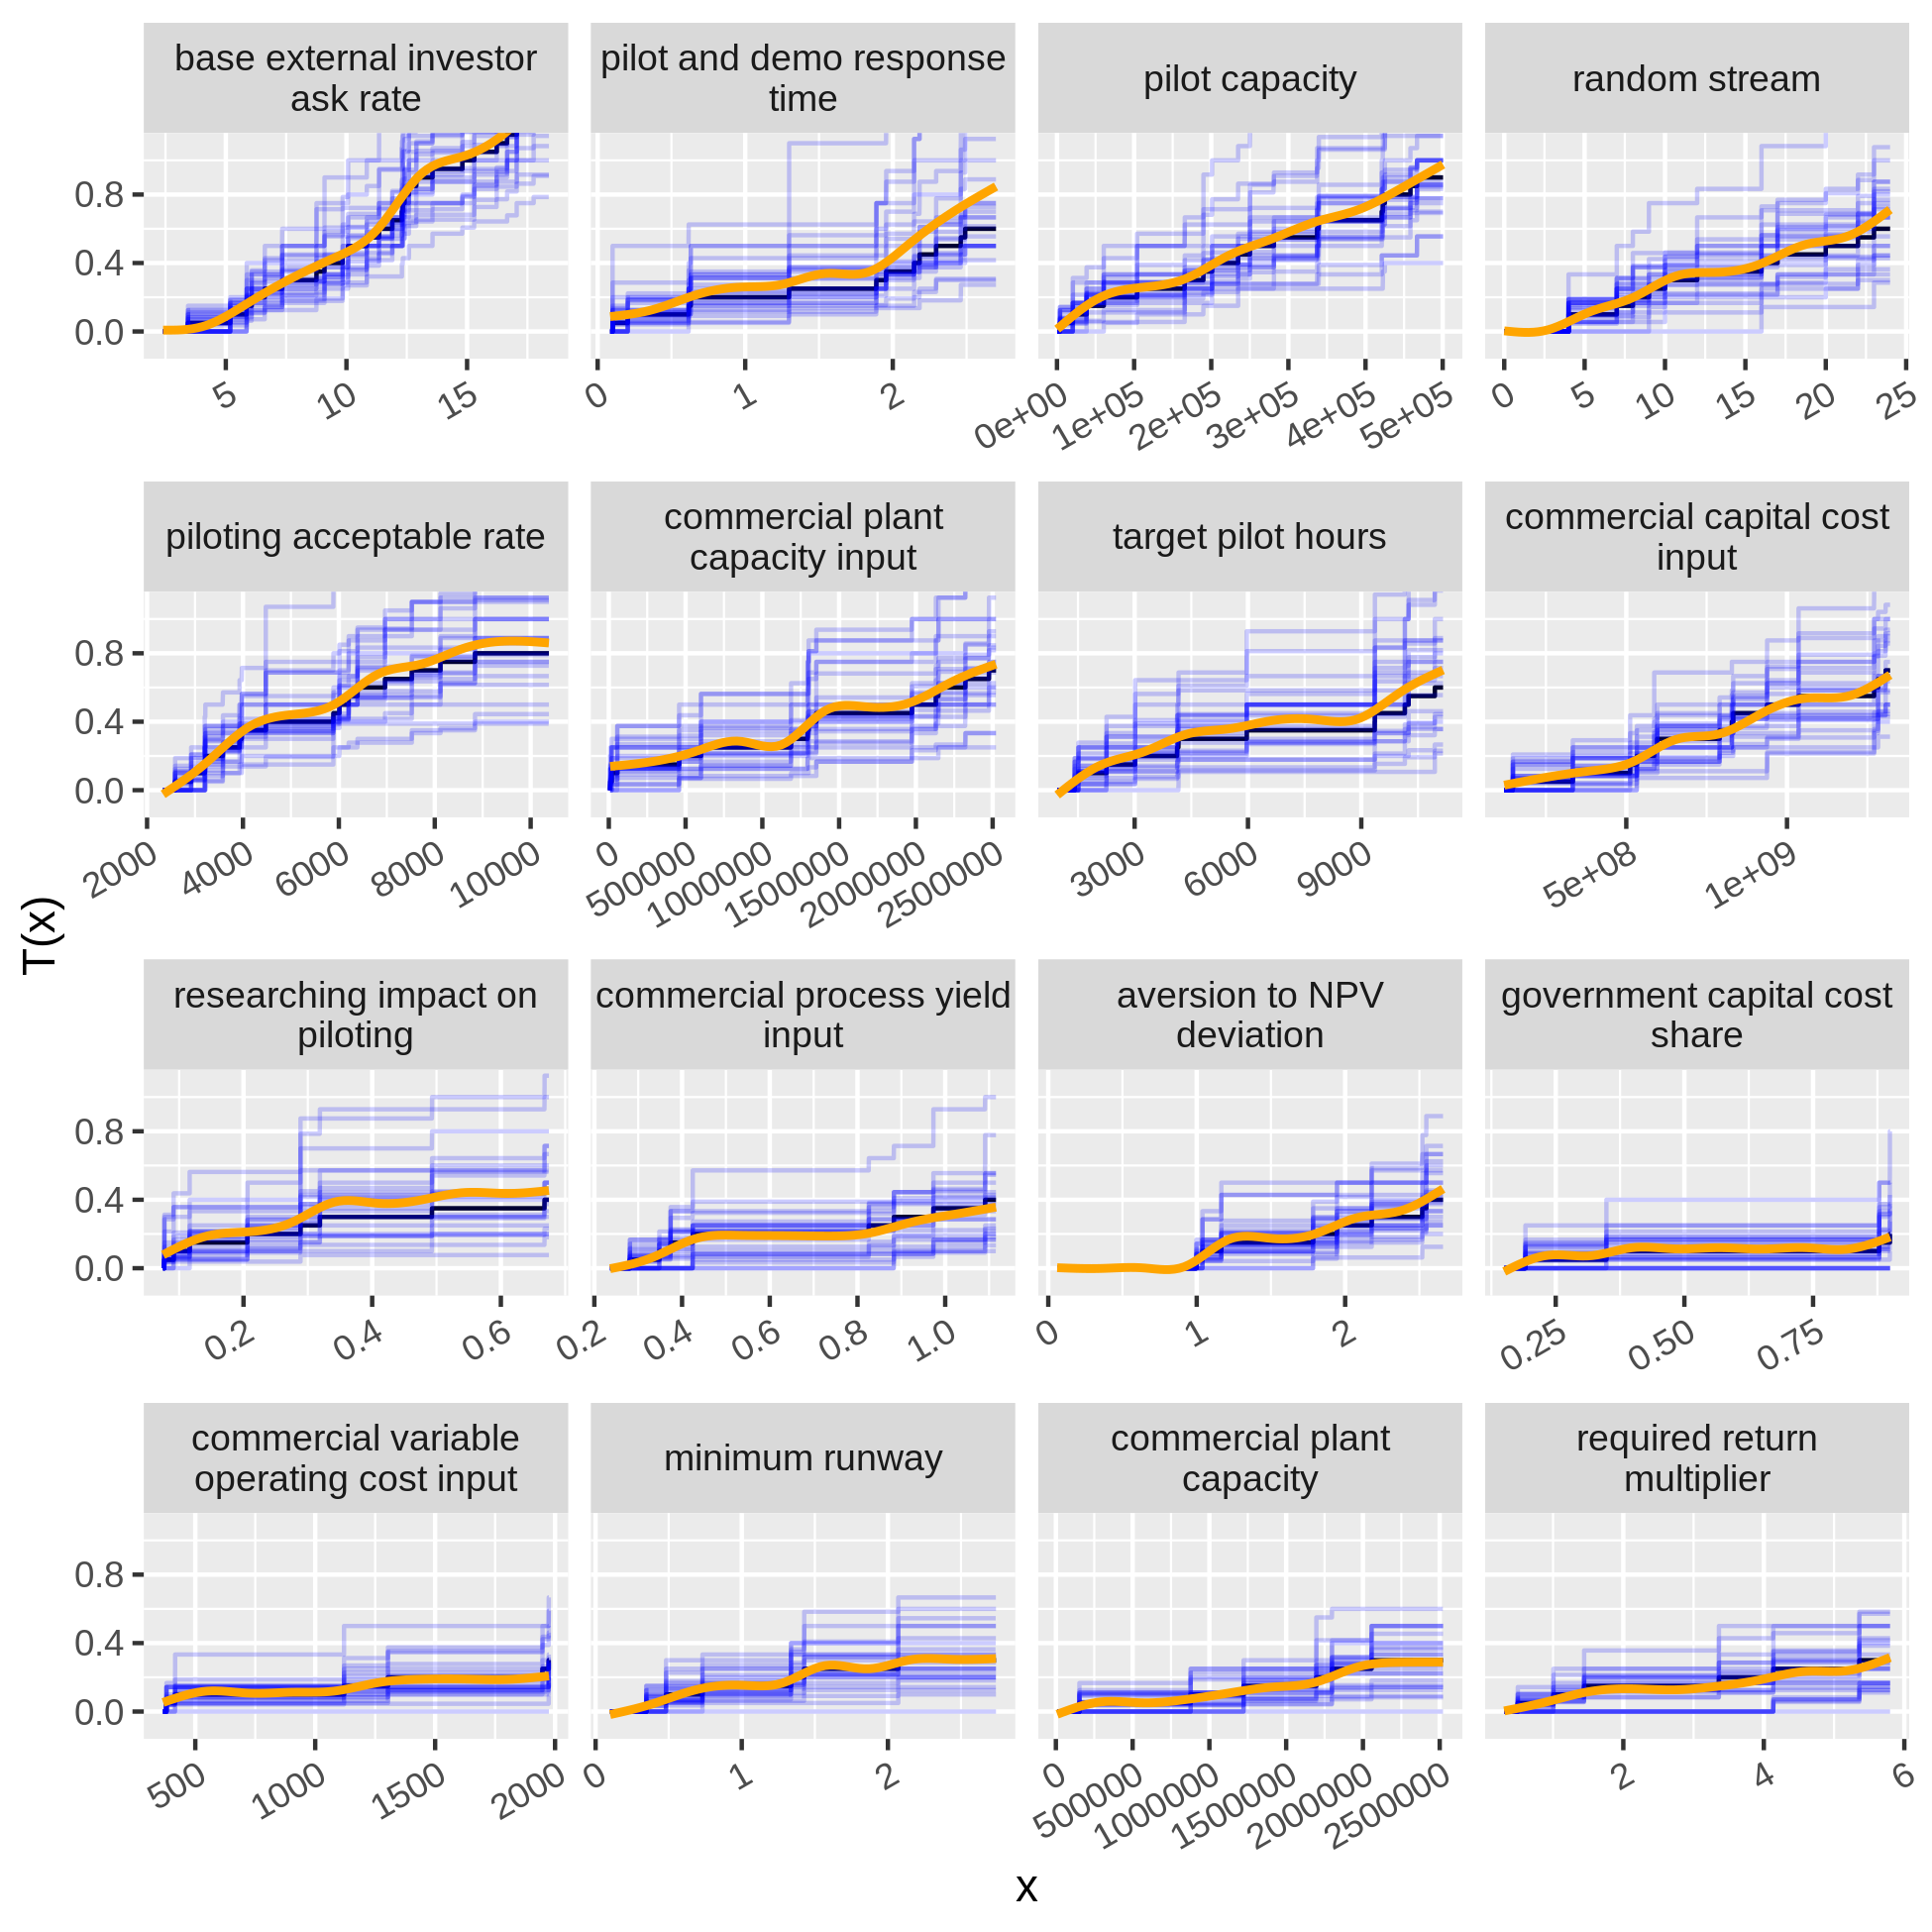
\includegraphics[width=\linewidth]{figures/btd-t.png}
    \caption{Cumulative local sensitivity $T_{i,j}^{(2,\epsilon)}(x)$ for the BTD model, with $j =$ ``demo plant construction'' and $N = M = 2500$. The black curve is the computed sensitivity, the 25 blue curves are sensitivities obtained by resampling the observations, and the orange curve is the fit from a general additive model for the blue curves.}
    \label{fig:btd-t}
\end{figure}

\begin{figure}
    \centering
    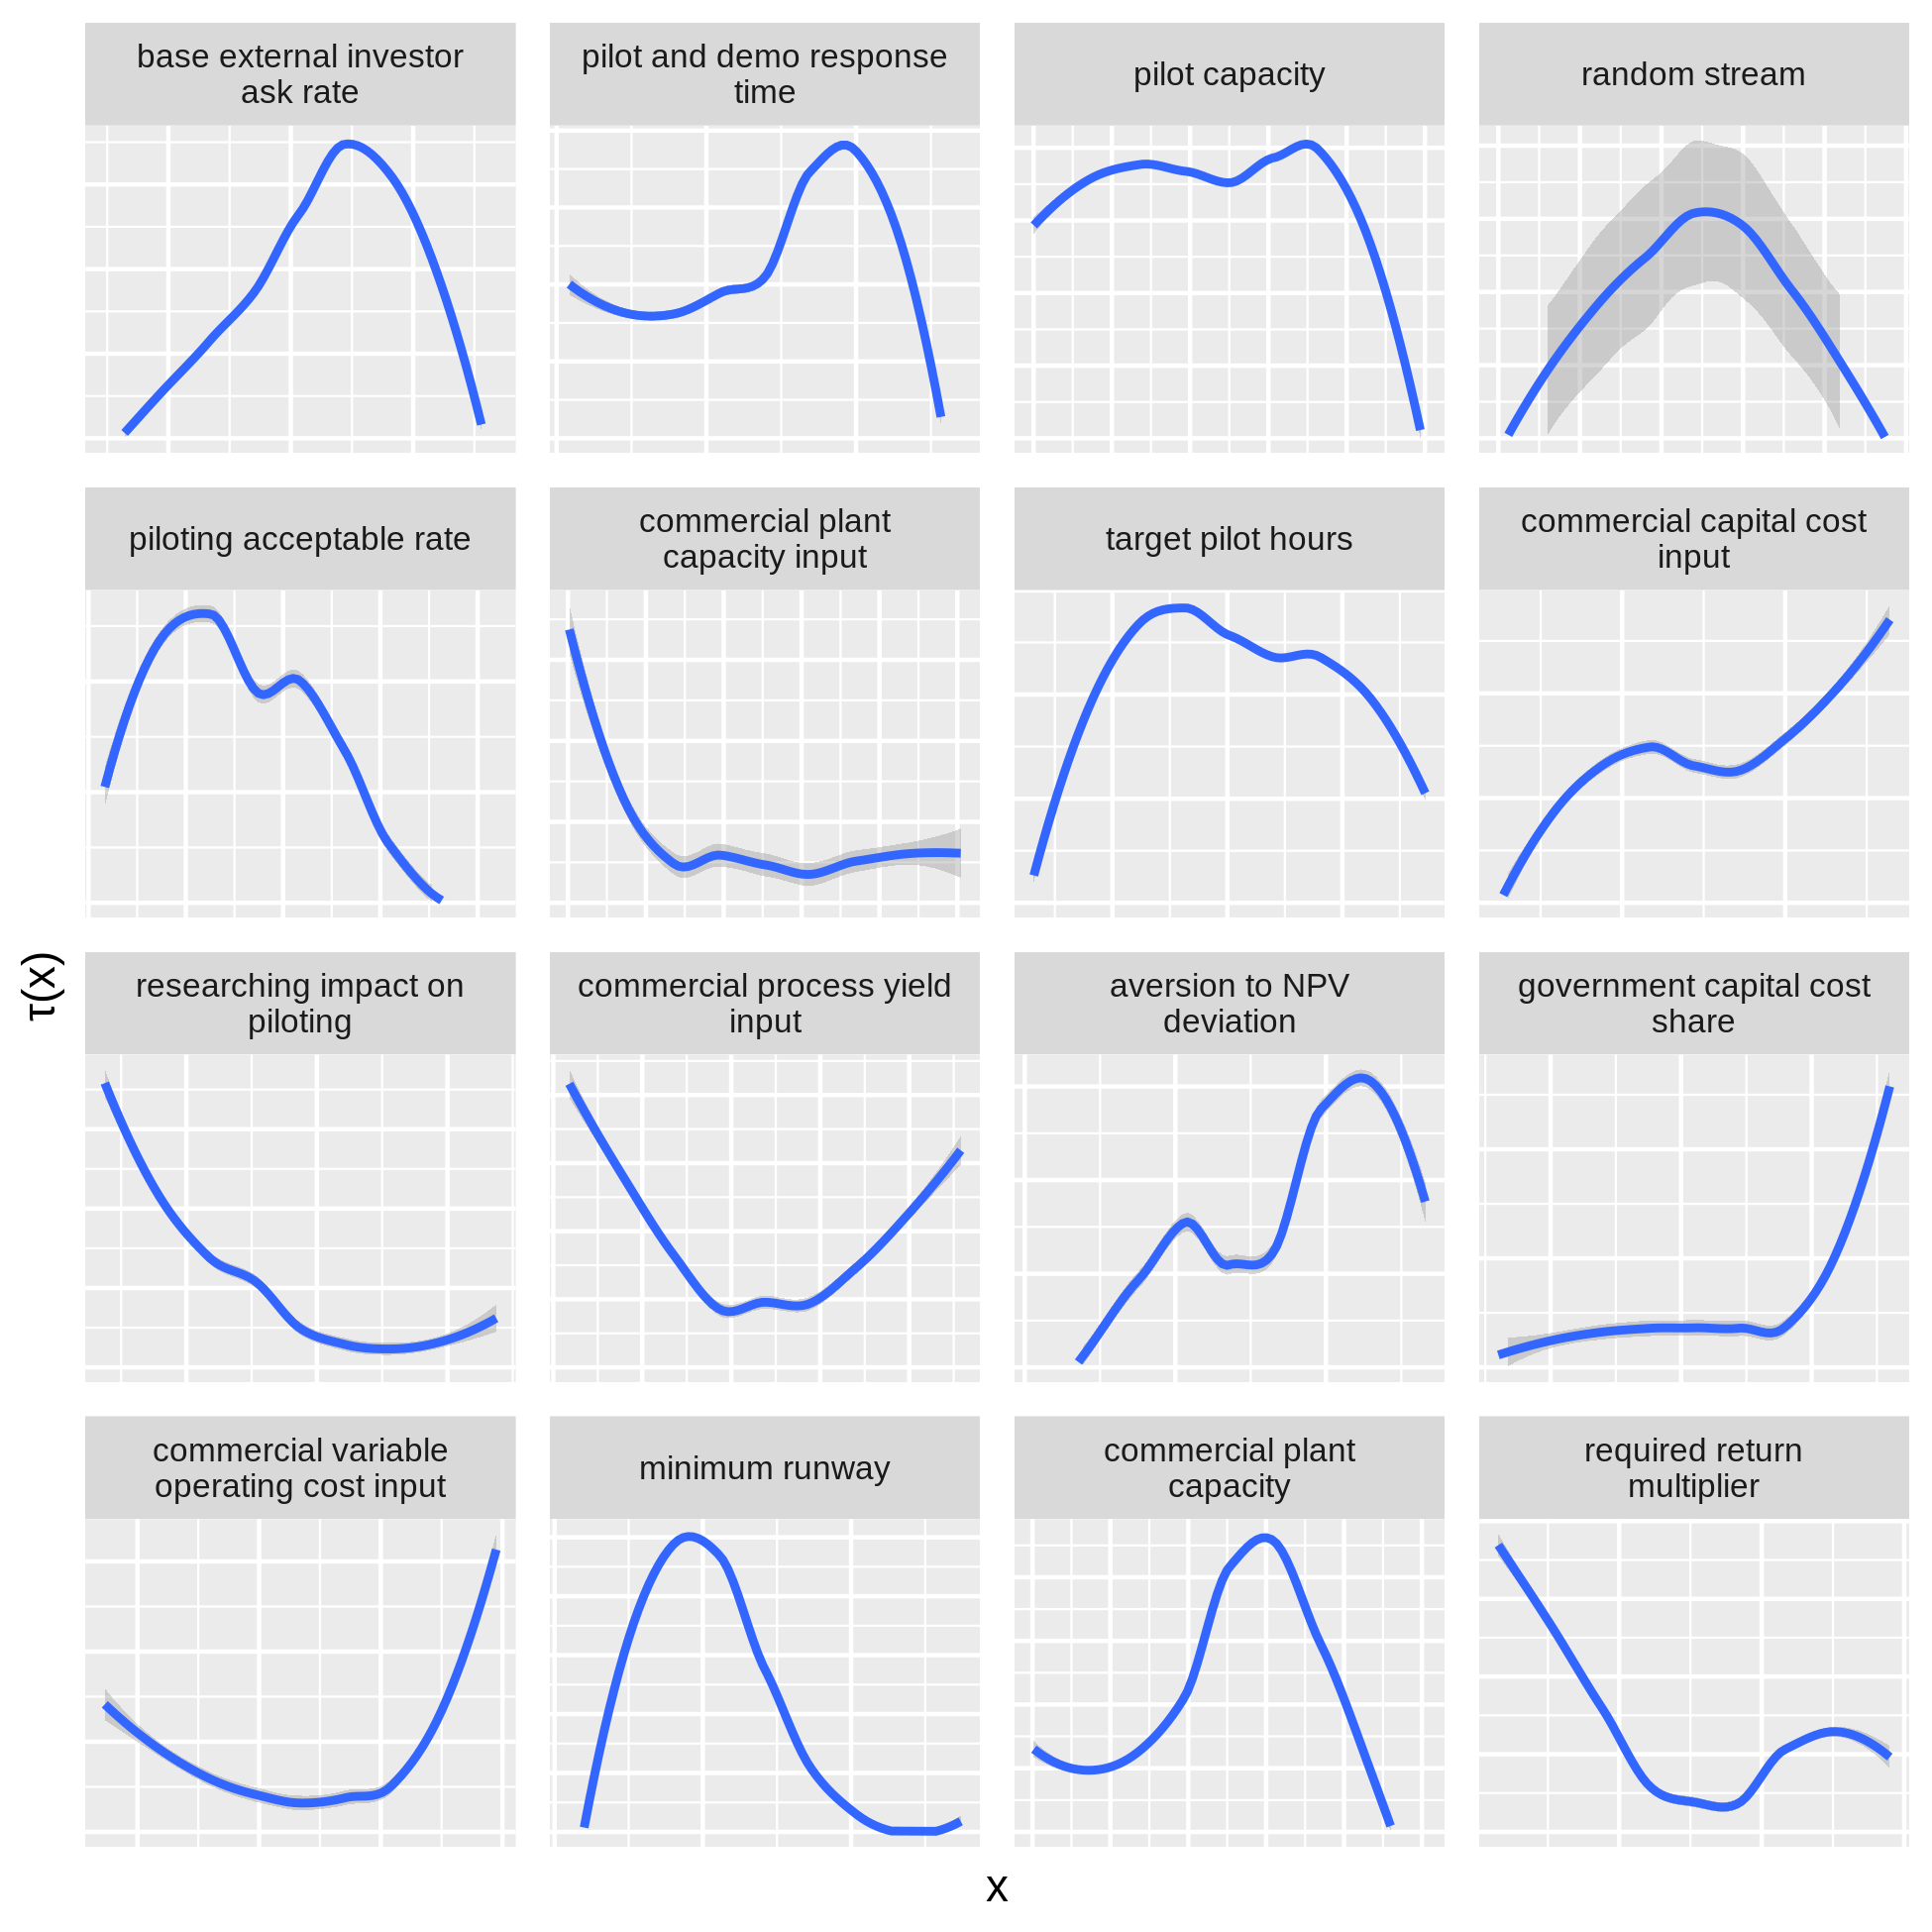
\includegraphics[width=\linewidth]{figures/btd-tau.png}
    \caption{Sensitivity density $\tau_{i,j}^{(2,\epsilon)}(x)$ for the BTD model, with $j =$ ``demo plant construction'' and $N = M = 2500$. (Note that the density is smoothed using LOESS, with dark gray bands for the confidence interval of the smoothed curve.)}
    \label{fig:btd-tau}
\end{figure}

\begin{figure}
    \centering
    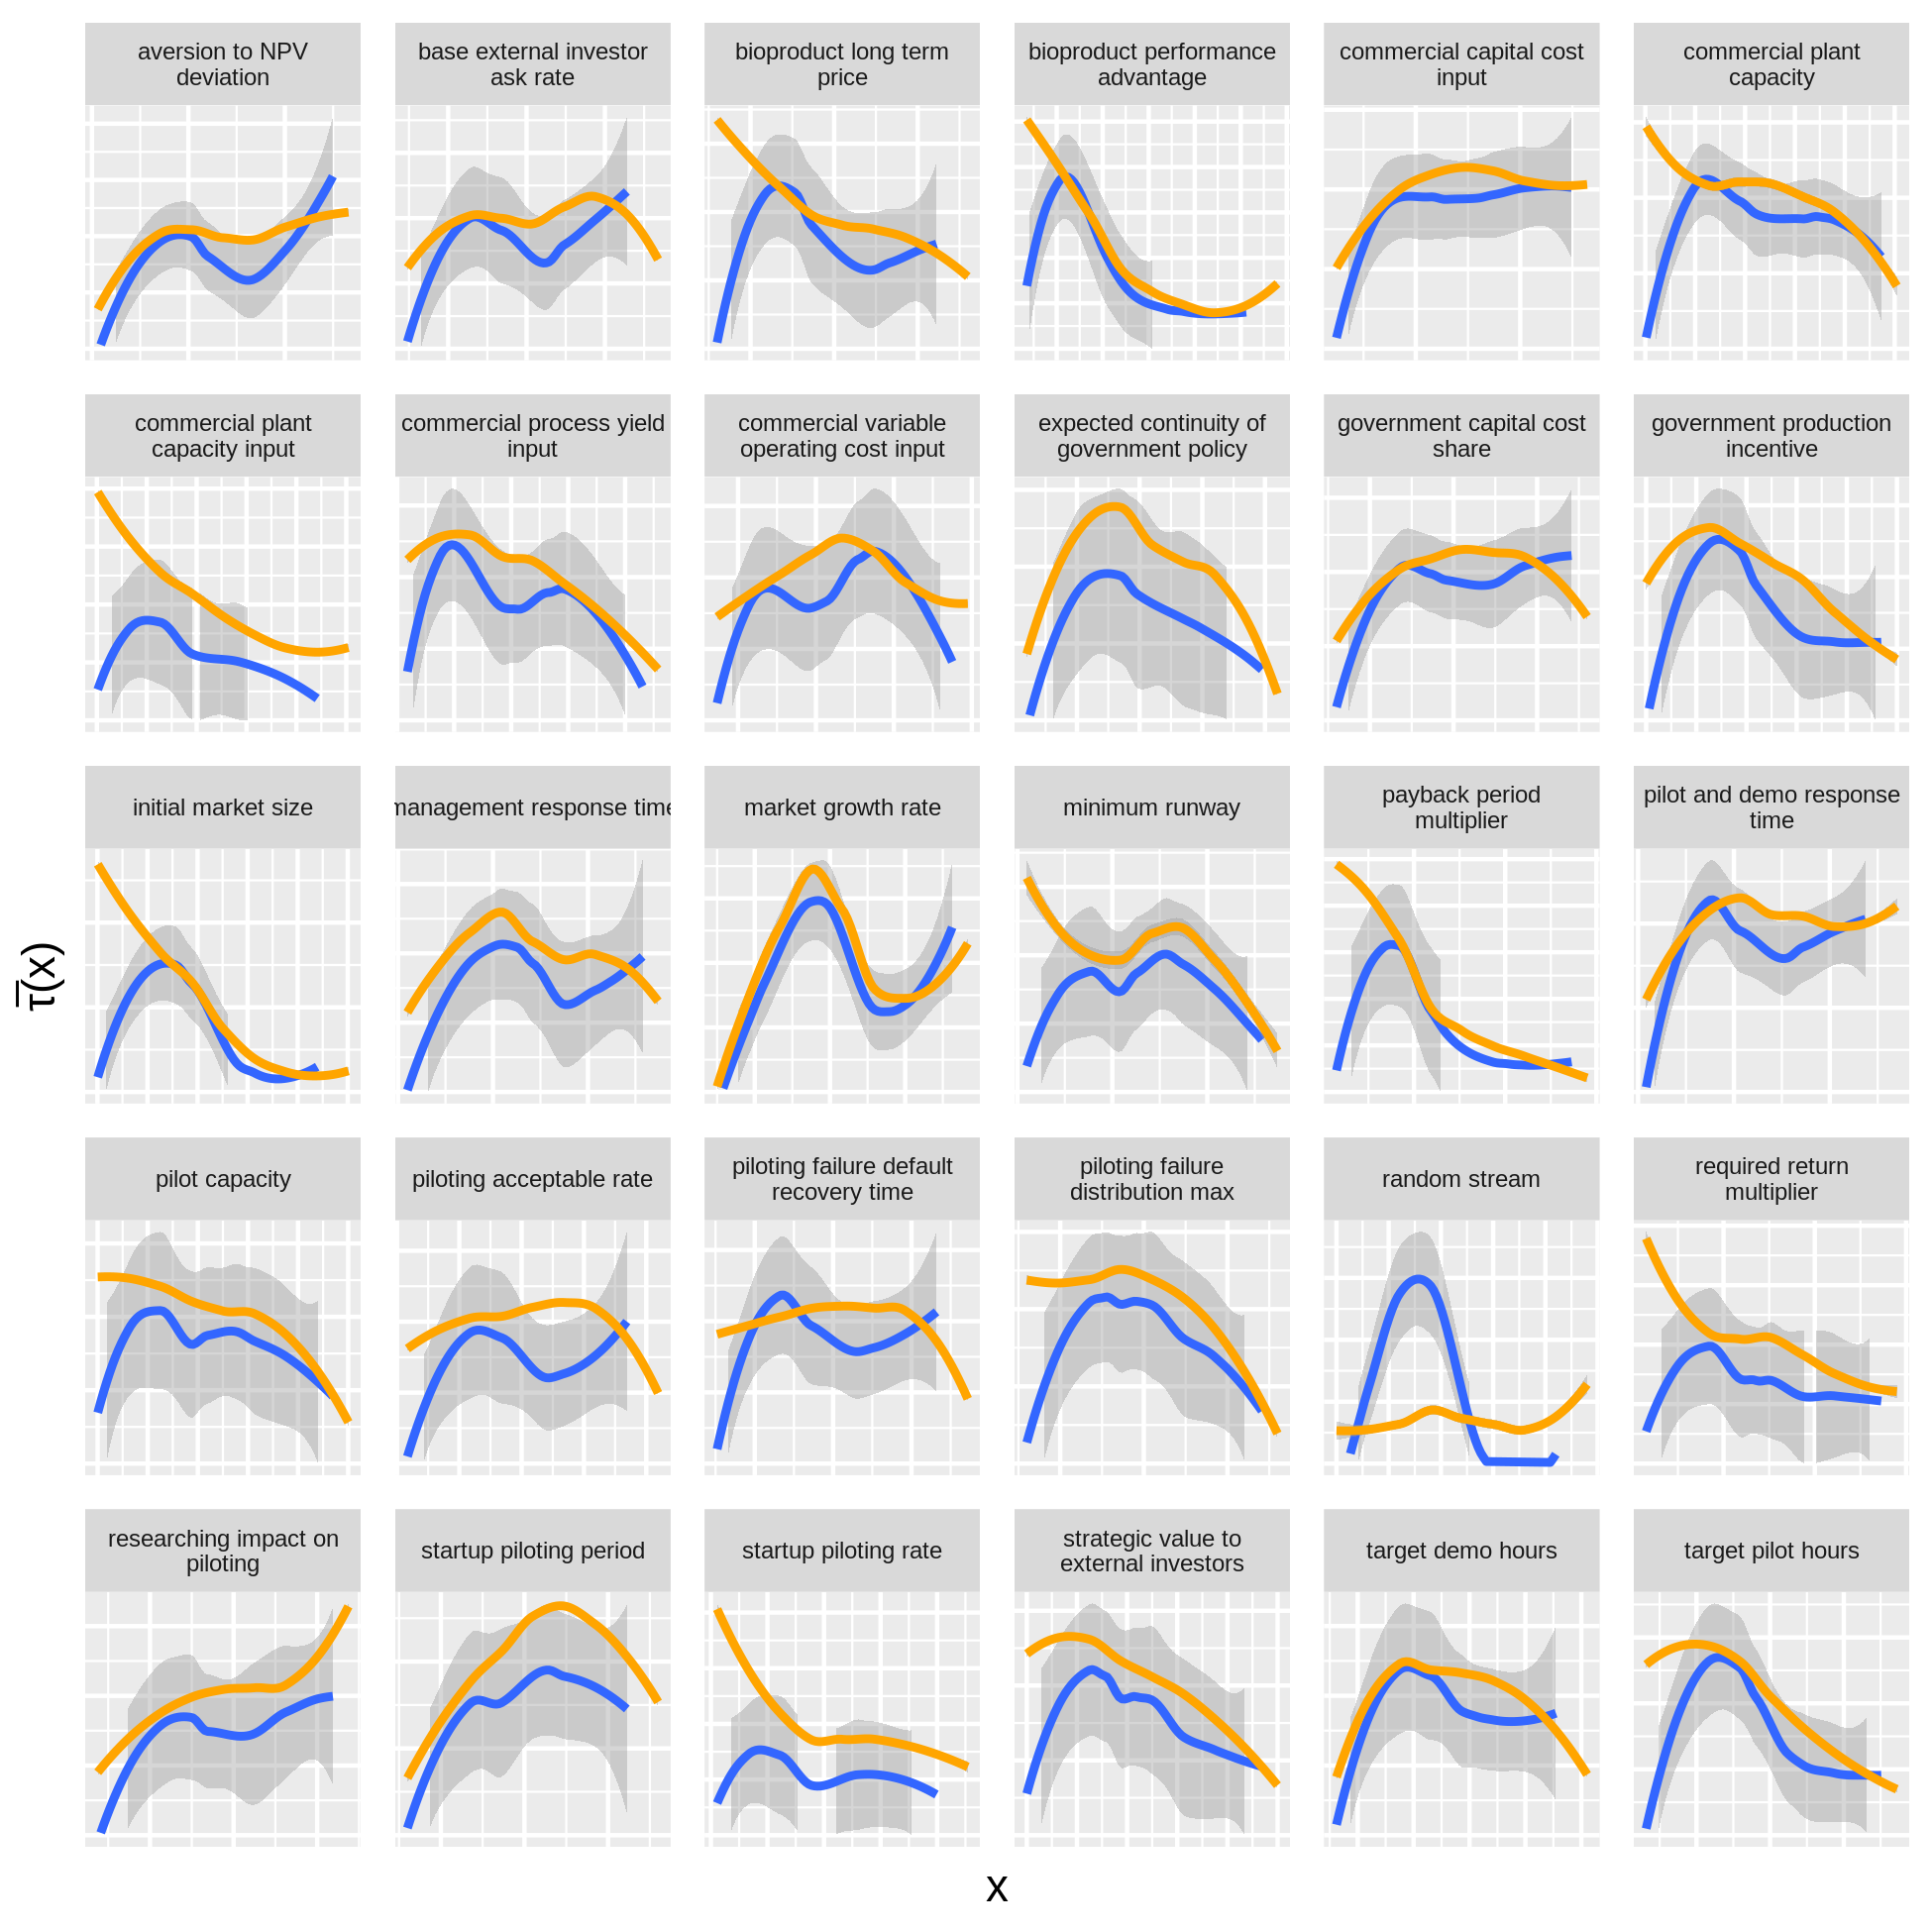
\includegraphics[width=\linewidth]{figures/btd-taubar1.png}
    \caption{Average sensitivity density $\overline{\tau}_i^{(2,\epsilon)}(x)$ for the BTD model, for the first batch $N = M = 10$ observations (blue with dark gray) and for the full set of $N = 2500$ observations (orange). (Note that the density is smoothed using LOESS, with dark gray bands for the confidence interval of the smoothed curve.)}
    \label{fig:btd-taubar1}
\end{figure}


\section{Conclusion}

\todo{PCA could be applied on the input space, too, or tensor PCA (maybe functional tensor PCA) could be employed.}


\section*{Acknowledgements}

This work was authored in part by the National Renewable Energy Laboratory, operated by Alliance for Sustainable Energy, LLC, for the U.S. Department of Energy (DOE) under Contract No. DE-AC36-08GO28308. Funding provided by the Department of Energy Office of Energy Efficiency and Renewable Energy Bioenergy Technologies Office. The views expressed in the article do not necessarily represent the views of the DOE or the U.S.\ Government. The U.S.\ Government retains and the publisher, by accepting the article for publication, acknowledges that the U.S.\ Government retains a nonexclusive, paid-up, irrevocable, worldwide license to publish or reproduce the published form of this work, or allow others to do so, for U.S. Government purposes.


% FIXME: Remove this.
\nocite{*}


\printbibliography


\appendix


\section{Toy Model}
\label{sec:toy}

This toy model consists of a nonlinear ordinary differential equation for $y_j$ as a function of $x_i$, with $i \in \{ 1 \ldots m \}$ and $j \in \{ 1 \ldots n \}$:
\begin{equation*}
    \frac{dy}{dt} = \kappa \cdot y \ z \ \left( 1 - \sigma \cdot y \  z \right) ,
\end{equation*}
where
\begin{equation*}
    z_j = \sum_{i=1}^m \mathbbm{1}_{j \in L_i} \mathbbm{1}_{x_i \ge \xi_i} \zeta_i \left( x_i - \xi_i \right)^{\delta_i} .
\end{equation*}
The parameters $\xi_i$ define locations of discontinuities and the parameters $\delta_i$ specify the degree of those discontinuities. The parameters $L_i$ affect the mixing of the input variables into the output, as do the matrices $\kappa$ and $\sigma$. The model was designed to exhibit nontrivial and nonlinear behavior with tunable discontinuous behavior. It can be used as a timeseries generator or just evaluated at a specified final time.

The particular instantiation of the toy model studied in this paper uses the following parameter values:
\begin{align*}
    m & = 3
    \\
    n & = 3
    \\
    t & \in [0, 10]
    \\
    L & = \begin{bmatrix} \left\{ 2, 3 \right\} & \left\{ 1, 2 \right\} & \left\{ 1, 2, 3 \right\} \end{bmatrix}
    \\
    \delta & = \begin{bmatrix} 0 & 1 & 2 \end{bmatrix}
    \\
    \xi & = \begin{bmatrix} 0.5933 & 0.9485 & 0.1030 \end{bmatrix}
    \\
    \zeta & = \begin{bmatrix} 0.8788 & 0.2668 & 0.6661 \end{bmatrix}
    \\
    y(0) & = \begin{bmatrix} -0.1900 & 0.5145 & 0.4094 \end{bmatrix}
    \\
    \kappa & = \begin{bmatrix} 0.7054 & 0.2921 & 0.7361 \\ -0.1151 & 0.5206 & -0.0707 \\ 0.3475 & -0.0579 & -0.2229 \end{bmatrix}
    \\
    \sigma & = \begin{bmatrix} 0.0294 & 0.1668 & 0.5788 \\ 0.1046 & 0.1705 & 0.2749 \\ -0.1258 & -0.0712 & 0.7372 \end{bmatrix}
\end{align*}

The following R code implements this toy model:

\begin{small}
\begin{verbatim}
# Create a multivariate function with specified properties:
#   tmax: maximum time
#   multiplicities: number of correlations each parameter has
#   degrees: polynomial degree of each parameter
#   dimension: the dimension of the output
#   returns a multivariate function of the vector of parameters and time
makeGenerator <- function(multiplicities, degrees, dimension) {
    single <- function(degree) {
      x0 <- runif(1)
      z0 <- runif(1)
      print(paste("Critical point at x = ", x0, sep = ""))
      function(x) {
          if (x < x0)
              0
          else
              z0 * (x - x0)^degree
      }
    }
    locations <- lapply(
        multiplicities,
        function(m) sample(1:dimension, m)
    )
    functions <- lapply(degrees, single)
    start <- runif(dimension, -0.25, 0.75)
    coefs <- matrix(
        runif(dimension^2, -0.25, 0.75),
        dimension,
        dimension
    )    
    shift <- matrix(
        runif(dimension^2, -0.25, 0.75),
        dimension,
        dimension
    )
    function(x, ts) {
        z <- rep(0, dimension)
        for (i in 1:length(locations))
            for (j in locations[[i]])
                z[j] <- z[j] + functions[[i]](x[i])
        ode(start, ts, function(t, y, params) {list((coefs %*% y) * z *
            (1 - ((shift %*% y) * z)))})
    }
}
\end{verbatim}
\end{small}

Here is a simple example of the use of this function:
\begin{small}
\begin{verbatim}
# Use reproducible random numbers.
RNGkind("Mersenne-Twister", "Inversion", "Rejection")
set.seed(46)

# Instantiate the model.
f <- makeGenerator(c(2, 2, 3), c(0, 1, 2), 3)
#   "Critical point at x = 0.593385165324435"
#   "Critical point at x = 0.948547213338315"
#   "Critical point at x = 0.102978735696524"

# Evaluate it at x = (0.1, 0.2, 0.3) for t = 0, 5, 10.
f(c(0.1, 0.2, 0.3), c(0, 5, 10))
# time    1          2          3
# 0     -0.1900320  0.5144967  0.4093612
# 5     -0.1478757  0.5489932  0.3864914
#10     -0.1024813  0.5854096  0.3659173
\end{verbatim}
\end{small}


\end{document}
